% CV in LaTeX
\documentclass[10pt]{article} % article with 12pt font
%% PACKAGES %%

\usepackage[english]{babel} % multilingual support
\usepackage[utf8]{inputenc} % encoding
\usepackage{blindtext} % to insert blind text
\usepackage{amsmath,amssymb,amsfonts}
\usepackage{amsthm}
\usepackage{soul}

\usepackage{geometry}
\geometry{
	a4paper,
	left=10mm,
	right=10mm,
	bottom=10mm,
	top=10mm}
% empty the headers, footers, page numbers…
\pagestyle{empty}
% Custom sectioning with secsty
\usepackage{sectsty}

\sectionfont{%                        
	\large % make sections smaller
	\fontfamily{qag}\selectfont % change font family
	\sectionrule{0pt}{0pt}{-5pt}{1pt} % insert a thin rule
}

\usepackage[shortlabels]{enumitem}% http://ctan.org/pkg/enumitem
% \setlist[itemize]{noitemsep, topsep=0pt}
\newlist{tabitemize}{itemize}{1}
\newlist{soloitemize}{itemize}{1}
\setlist[tabitemize,soloitemize]{
	nosep, nolistsep,
	topsep=0pt,
	itemsep=3pt,
	align=left,
	left=2pt,
	label=$\bullet$,
}

\usepackage[absolute,overlay]{textpos}  % For positioning the box
\usepackage{calc}
\usepackage[shortcuts]{extdash}
\usepackage{graphicx} 
\usepackage{longtable}

\usepackage{color}



%\reversemarginpar

\usepackage[most]{tcolorbox}
\usepackage{xcolor}
\usepackage{lipsum} % for example text

\definecolor{myhlcolor}{HTML}{fbff8b}  % equivalent to #FF8800
\sethlcolor{myhlcolor}

\definecolor{myurlcolor}{HTML}{6997ff} 


\usepackage[colorlinks=true, linkcolor=black, urlcolor=black, citecolor=black, pdfborder={0 0 0}]{hyperref}
\usepackage[normalem]{ulem}  % để dùng \uline cho gạch chân

% Định nghĩa lại \href để gạch chân link
\let\oldhref\href
\renewcommand{\href}[2]{\oldhref{#1}{\uline{#2}}}


%% MACROS %%

% size of the boxes used to align text
\newlength{\spacebox}
\settowidth{\spacebox}{123456789}
% vertical space separator between entries

\usepackage{tikz}      % for drawing dashed lines

\newcommand{\sepspace}{%
	\par\vspace{0.5em} % optional vertical spacing before line
	\noindent
	\tikz{\draw[gray, dashed, line width=0.5pt] (0,0) -- (\linewidth,0);}%
	\par\vspace{0.5em} % optional vertical spacing after line
}

% name
\newcommand{\name}[1]{
	\Huge % font size
	\fontfamily{phv}\selectfont % font family
	% print name centered and bold
	%\begin{center} 
		\textbf{#1} 
	%\end{center}
	\par
	% back to normal size and font
	\normalsize\normalfont}

% subnam
\newcommand{\subname}[1]{
	\large % font size
	\fontfamily{phv}\selectfont % font family
	% print subname centered and slanted
	%\begin{center} 
		\textsl{#1}
		%\end{center}
		\par
	% back to normal size and font
	\normalsize \normalfont}


% motto
\newcommand{\motto}[1]{
	% \large % font size
	\fontfamily{phv}\selectfont % font family
	% print motto centered and slanted
	\begin{center} \textsl{#1}\end{center}\par
	% back to normal size and font
	\normalsize \normalfont}

% personal information
\newcommand{\info}[2]{
	% set specific indentation for personal information
	% \fontfamily{phv}\selectfont
	\noindent\hangindent=2em\hangafter=0
	% create a box to align two pieces of text
	\parbox{\spacebox}{%
		\textsl{#1}} % slanted entry name
	#2 \par} % entry value



% skill
\newcommand{\skill}[2]{
	% set specific indentation for personal information
	\noindent\hangindent=1em\hangafter=0
	% create a box to align two pieces of text
	\parbox{2.5\spacebox}{% three times larger box
		\textbf{{#1}}} % small caps entry name
	#2 \par \vspace{0.15cm}} % entry value




% education entry
\newcommand{\education}[4]{
	\noindent  {\textbf{#1}} \textit{(#2)}
		\par
	\noindent \textit{#3} \par
	\vspace*{0.5em}
	\noindent\hangindent=2em\hangafter=0  #4 
	\normalsize \par}


% work experience
\newcommand{\work}[4]{
	\noindent  {\textbf{#1}} \textit{(#2)}
	\par
	\vspace*{0.5em}
	\noindent \textit{#3} \par
	\vspace*{0.5em}
	\noindent\hangindent=2em\hangafter=0  #4 
	\normalsize \par}
	
	
% publication entry
\newcommand{\publication}[6]{
	\noindent{\textbf{#1} \hspace{0.1cm} {#2}} (#3)
	\par
	\vspace*{0.5em}
	\noindent {#4} 
	\par
	\vspace*{0.5em}
	\noindent \textit{#5}
	\par
	\vspace*{0.5em}
	DOI: \href{https://doi.org/#6}{#6}
	\normalsize \par}
	
	
	
% conference entry
\newcommand{\conferece}[2]{
	\noindent{\textbf{#1}}
	\par
	\vspace*{0.5em}
	\noindent {#2} 
	\normalsize}


% conference entry
\newcommand{\award}[2]{
	\noindent{\textbf{#1}}
	\par
	\vspace*{0.5em}
	\noindent {#2} 
	\normalsize}
	
	
%
%\definecolor{TitleColor}{HTML}{4C0099}
%\definecolor{SubTitleColor}{HTML}{0000CC}
\definecolor{TitleColor}{HTML}{000000}
\definecolor{SubTitleColor}{HTML}{000000}

\usepackage{wasysym} % Load the smiley package

\begin{document}
	
	
	% Create a box in the top-right corner
	\begin{textblock*}{5cm}(15.5cm,0.3cm) % Adjust the position and size as needed\
		\centering
		\begin{tcolorbox}[colframe=black, colback=white, sharp corners]
			\fontfamily{phv}\selectfont \centering\footnotesize \textit{Last update: May 2025} \normalsize\normalfont
		\end{tcolorbox}
	\end{textblock*}
	
	
	% \begin{textblock*}{10cm}(9cm,29cm) % Adjust the position and size as needed\
		%     \centering 
		%     \textit{This CV has been prepared to be sent to \_\_\_\_\_\_\_\_\_\_\_\_\_\_\_\_\_\_}
		% \end{textblock*}
	
	% \begin{textblock*}{4.5cm}(16.5cm, 6cm) % Adjust the position and size as needed\
		%     \centering
		%     \includegraphics[height = 2.5cm]{qr_code_resume.png}
		% \end{textblock*}
	
	
	% name and motto
	\name{\color{TitleColor}Duc-Cuong VU, BcS.}
	%\subname{\color{TitleColor}Bachelor of Science in Automation and Control}
	% \vspace*{-5pt}
	% \motto{``I am interested in Automation, Mechatronics, Robotics, Nonlinear Control, Modeling and Simulation, Electrical-Electronic and Experiment systems''}
	
	% personal information
	\sepspace
	\info{Email}{\href{mailto:vdcuong2002@gmail.com}{\texttt{vdcuong2002 [at] gmail.com}}}
	\info{Phone}{+84 865 280 802}
	\info{Address}{Giao Thuy, Nam Dinh, Vietnam}
	\info{Sites}{\href{https://dc-vu.github.io}{https://dc-vu.github.io}}
	
	% education
	
	
	\section*{\color{TitleColor}Education}
	
	\education{Master of Science in Automation and Control}{Jul 2024 - present}{School of Electrical - Electronics Engineering, \\Hanoi University of Science and Technology (HUST), Hanoi, Vietnam}
	{
		\begin{soloitemize}
			\item \textbf{Research project:} \textit{Design control structures for Parallel Platforms in Maritime applications}
			\item \textbf{Funded by:} \textit{Master, PhD Scholarship Programme of Vingroup Innovation Foundation (VINIF)} 
		\end{soloitemize}
	}
	\sepspace
	
	\education{Bachelor of Science in Automation and Control}{Oct 2020 - Mar 2024}{School of Electrical - Electronics Engineering, \\Hanoi University of Science and Technology (HUST), Hanoi, Vietnam}
	{\begin{soloitemize}
			\item \textbf{Excellent degree}, GPA: 3.71/4. Finished the 4-year BSc program in \textbf{just 3.5 years}.
			\item \textbf{Ranking:} 27/499 in the same cohort.
			\item \textbf{Bachelor Thesis:} \textit{Balancing, motion planning, and tracking control for ballbot systems}. \\
			\textbf{Thesis score:} 9.9/10 - The best thesis defense
		\end{soloitemize}
	}
	
	
	
	% work experience
	\section*{\color{TitleColor}Work Experience}
	
	\work{Research Assistant}{Oct 2021 - present}{The Mechatronics Engineering Group, \\School of Electrical - Electronic Engineering,\\Hanoi University of Science and Technology (HUST), Hanoi, Vietnam}{ \begin{soloitemize}
			\item \textbf{Research topics:} Automation, Control Design, Robotics, Multi-agent Systems, Modeling and Simulation, Experiment systems.
			\item \textbf{Supervisor:} \href{https://scholar.google.com/citations?user=MlJ_2-wAAAAJ&hl=en}{Assoc.Prof.PhD. Tung Lam Nguyen}
			% , PhD. Danh Huy Nguyen , PhD. Thi Van Anh Nguyen  
			({\href{mailto:lam.nguyentung@hust.edu.vn}{\texttt{lam.nguyentung}}}
			% , {\href{mailto:huy.nguyendanh@hust.edu.vn}{\texttt{huy.nguyendanh}}}, {\href{mailto:anh.nguyenthivan1@hust.edu.vn}{\texttt{anh.nguyenthivan1}}} 
			\texttt{[at] hust.edu.com}).
			\item \textbf{Skills acquired:}  hardware design, numerical simulation and modeling, analysis, and interpretation of results, study conception, and design, draft manuscript preparation, ...
			% \item \textbf{Projets:} Generating trajectory and balancing control of technical systems
		\end{soloitemize}
	}
%	
%	
%	\section*{\color{TitleColor}Personal skills}
%	\skill{Languages}{English, B2. Experienced in academic writing.}
%	\skill{Office}{Proficient in \LaTeX, TikZ, good command in MS Office}
%	\skill{Coding}{Python and MATLAB for simulation, C/C++ for real-time purposes.}
%	\skill{Simulation}{MuJoCo and MATLAB Simulink, Simscape simulation}
%	\skill{Embedded Systems}{STM32, NI myRIO, TI C2000, Arduino, ...}
%	\skill{Misc.}{CasADI for nonlinear optimization, SolidWorks, Altium, Linux kernel for EtherCAT Servo control, \dots}
%	
	
	% work experience
	\section*{\color{TitleColor}Projects}
	\begin{minipage}{0.65\textwidth}
		\work{Member/Researcher}{Mar 2025 - Dec 2025}{Advanced Control of a Ship-Mounted Stewart Platform for Marine Applications}{\begin{soloitemize}
				\item Field: Marine Robotics and Control Systems.
				\item International Collaboration of Korea Institute of Science and Technology (KIST) and Institute for Control Engineering and Automation (ICEA, HUST).
				\item Supervisors: \href{https://scholar.google.com/citations?user=qyExc4QAAAAJ&hl=en}{PhD. Minh Nhat Vu} and \href{https://scholar.google.com/citations?user=MlJ_2-wAAAAJ&hl=en}{Assoc.Prof.PhD. Tung Lam Nguyen}
			\end{soloitemize}
		}
	\end{minipage}
	\hfill
	\begin{minipage}{0.33\textwidth}
		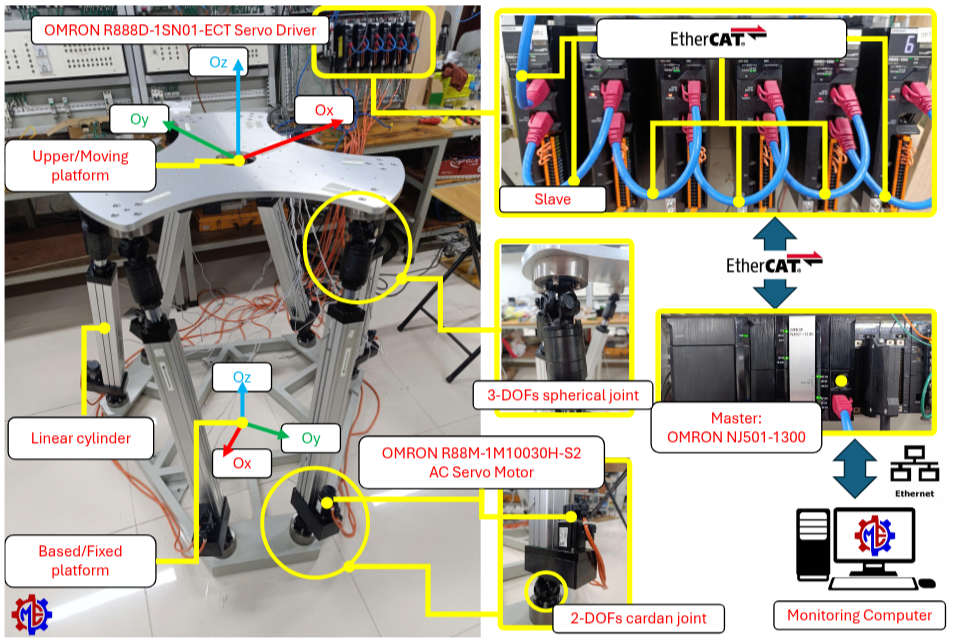
\includegraphics[width=\textwidth]{../images/hexapod.png}
	\end{minipage}
	
	\sepspace
	
	\noindent
	\begin{minipage}{0.65\textwidth}
		\work{Member/Researcher}{Jan 2025 - Dec 2027}{Robot navigation system integrating sensor network and wireless communication}{\begin{soloitemize}
				\item Field: Robotics and Control systems.
				\item Funded by Hanoi University of Science and Technology.
				\item Supervisors: \href{https://scholar.google.com/citations?user=mI561CkAAAAJ&hl=en}{PhD. Duc Chinh Hoang} and \href{https://scholar.google.com/citations?user=MlJ_2-wAAAAJ&hl=en}{Assoc.Prof.PhD. Tung Lam Nguyen}.
			\end{soloitemize}
		}
	\end{minipage}
	\hfill
	\begin{minipage}{0.33\textwidth}
		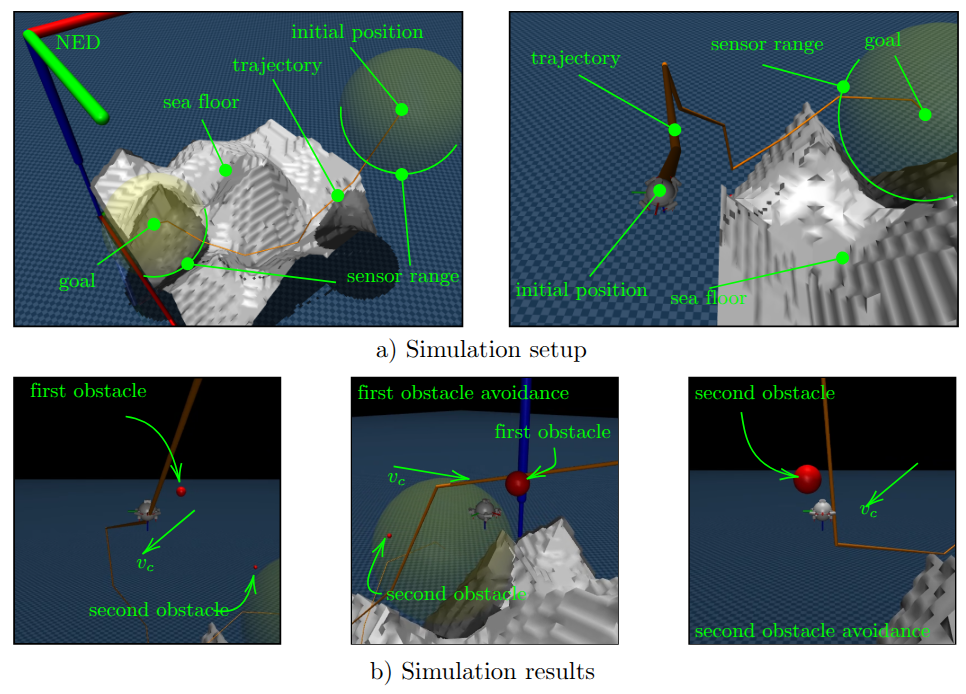
\includegraphics[width=\textwidth]{../images/ProjectTD.png}
	\end{minipage}
	
	
	
	\section*{\color{TitleColor}Highlighted Publications}
	
	\begin{minipage}{0.3\textwidth}
		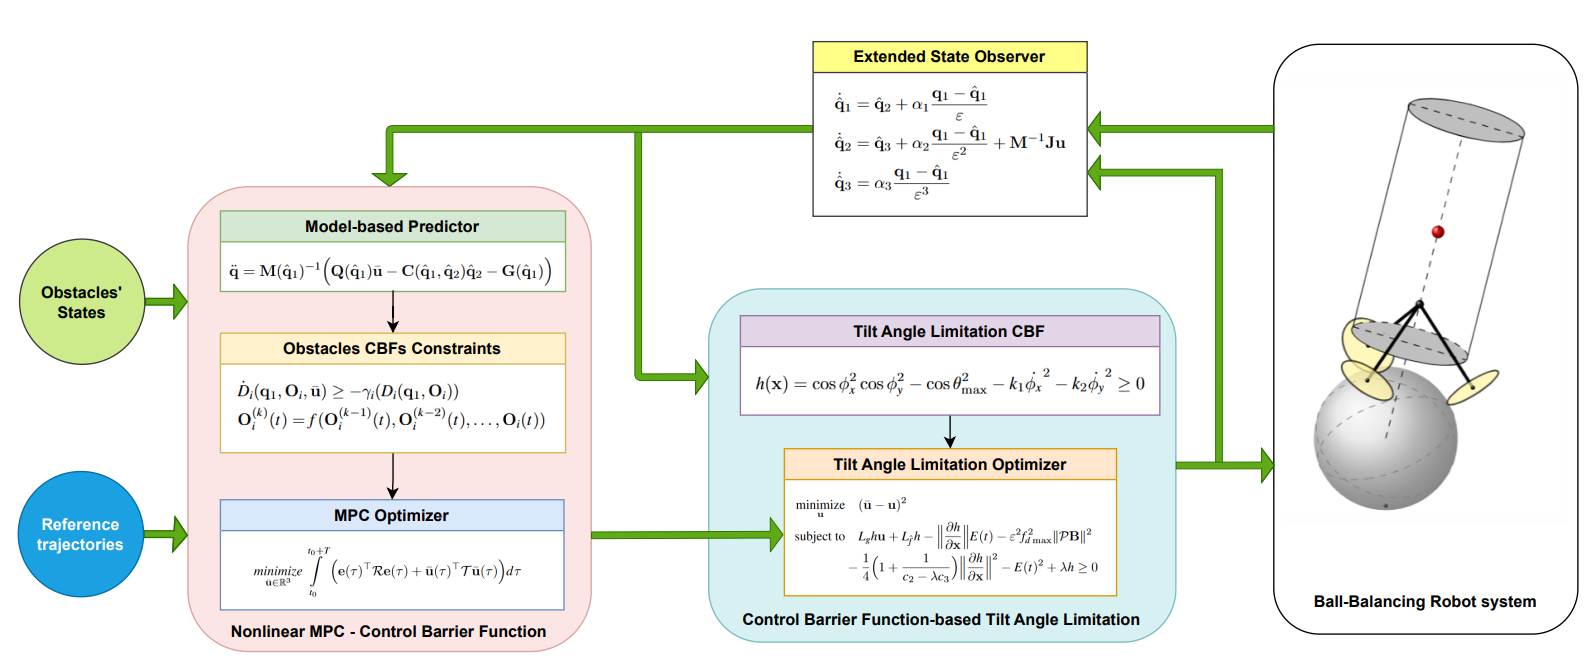
\includegraphics[width=\textwidth]{../images/IEEEAccess.png}
	\end{minipage}
	\hfill
	\begin{minipage}{0.68\textwidth}
		\publication{Journal}
		{IEEE Acess (ISI-Q2)}
		{2025}
		{CBFs-based Model Predictive Control for Obstacle Avoidance with Tilt Angle Limitation for Ball-Balancing Robots}
		{Minh Duc Pham, \hl{Duc Cuong Vu}, Thi Thuy Hang Nguyen, Thi Van Anh Nguyen, Minh Nhat Vu, and Tung Lam Nguyen}
		{10.1109/ACCESS.2025.3567474}
	\end{minipage}
	
	\sepspace
	\noindent
	\begin{minipage}{0.3\textwidth}
		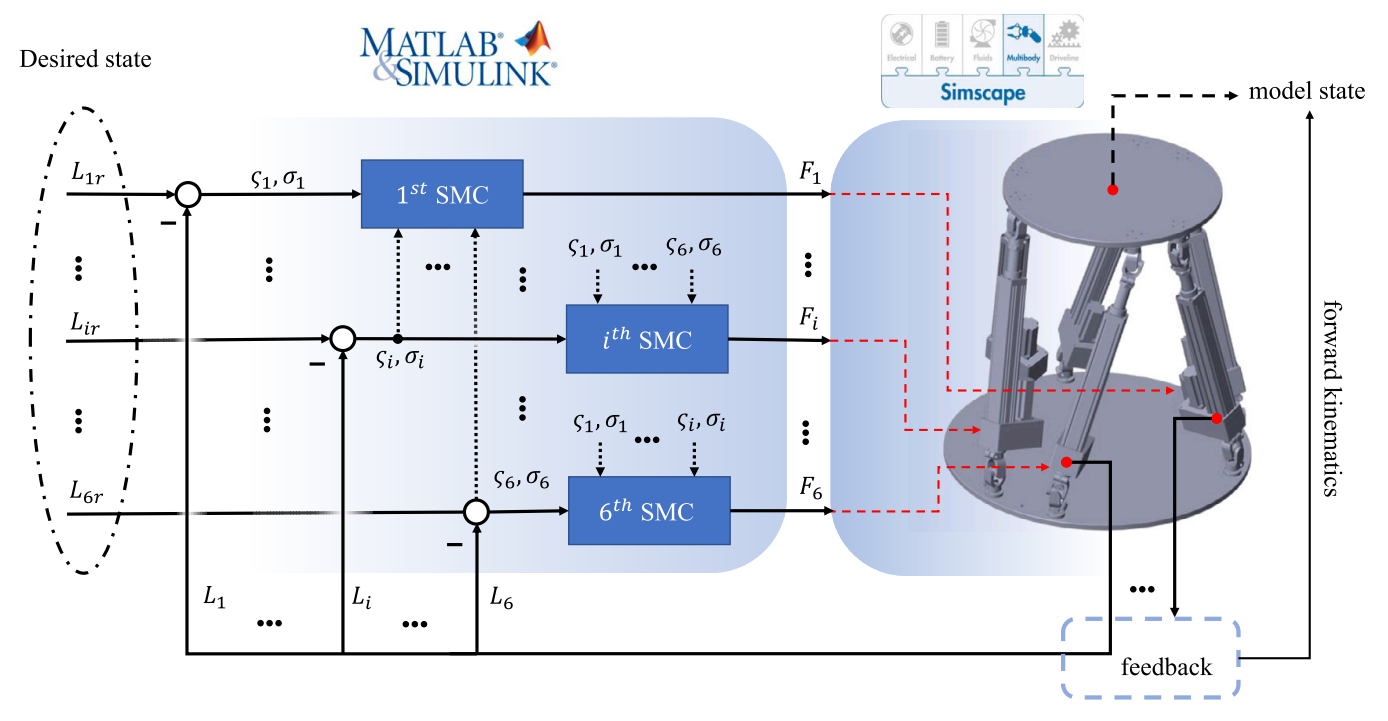
\includegraphics[width=\textwidth]{../images/RIENG.png}
	\end{minipage}
	\hfill
	\begin{minipage}{0.68\textwidth}
		\publication{Journal}
		{Results in Engineering (ISI-Q1)}
		{2025}
		{A novel approach of Consensus-based Finite-time Distributed Sliding Mode Control for Stewart platform manipulators motion tracking}
		{\hl{Duc Cuong Vu}, Danh Huy Nguyen, and Tung Lam Nguyen}
		{10.1016/j.rineng.2024.103872}
	\end{minipage}
	
	
	\sepspace
	\noindent
	\begin{minipage}{0.3\textwidth}
		\centering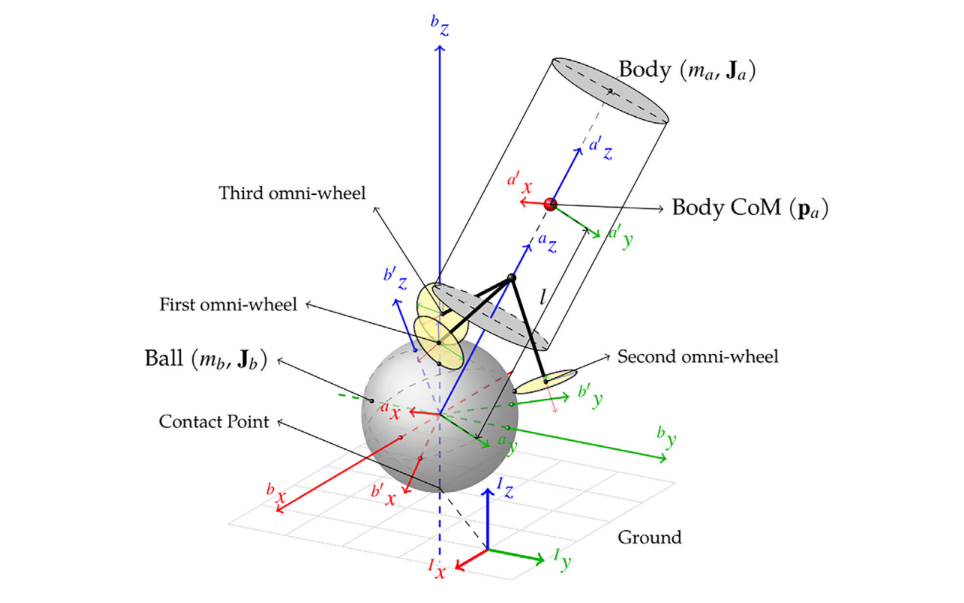
\includegraphics[width=0.8\textwidth]{../images/RNC.png}
	\end{minipage}
	\hfill
	\begin{minipage}{0.68\textwidth}
		\publication{Journal}
		{International Journal of Robust and Nonlinear Control (ISI-Q1)}
		{2024}
		{Time-optimal trajectory generation and observer-based hierarchical sliding mode control for ballbots with system constraints}
		{\hl{Duc Cuong Vu}, Minh Duc Pham, Thi Thuy Hang Nguyen, Thi Van Anh Nguyen, and Tung Lam Nguyen}
		{10.1002/rnc.7358}
	\end{minipage}
	
	
	
	\section*{\color{TitleColor}Conferences}
	\conferece{IEEE 12th International Conference on Control, Automation and Information Sciences (IEEE ICCAIS 2023)}
	{Hanoi, Vietnam}
	\sepspace
	\noindent\conferece{2024 International Conference on Advanced Technologies for Communications (ATC2024)}
	{Hanoi, Vietnam}
	\sepspace
	\noindent\conferece{International Conference on Intelligent Systems and Networks (Springer ICISN 2023)}
	{Hanoi, Vietnam}
	
	
	\section*{\color{TitleColor}Honours \& awards}
	\award{Master, PhD Scholarship Programme}{Vingroup Innovation Foundation (VINIF)}
	\sepspace
	\noindent
	\award{Best Thesis Defense Award}{Hanoi University of Science and Technology}
	
	
	
	% \section*{\color{TitleColor}My (funny) pictures and videos \smiley}
	% \includegraphics[width = 0.35\linewidth]{StewartPlatformWithMe.jpg} Duc Cuong VU and Stewart platform manipulator.
	
	% \par
	% \vspace{0.5cm}
	
	% \begin{soloitemize}
		%     \item Stewart platform videos: \texttt{\color{blue} https://youtu.be/73aYLjZv9QI}, \texttt{\color{blue}https://youtu.be/vGohLvgD4YA}
		%     \item Ball-balancing robot videos: \texttt{\color{blue}https://youtu.be/H8lpT75bVSM}, \texttt{\color{blue} https://youtu.be/TxwvtN1CRGk}
		% \end{soloitemize}
	
	% \par
	% \vspace{0.2cm}
	
	% \noindent\hangindent=2em \textbf{Best Paper} \quad {awarded by National Conference on Smart Technologies and Application for Industry 4.0, Smart City and Sustainability 2023}
	
	
	% \section*{\color{TitleColor}References}
	% \noindent\hangindent=2em \textbf{{Assoc.Prof.PhD. Tung Lam Nguyen}}, HUST, {\href{mailto:lam.nguyentung@hust.edu.vn}{\texttt{lam.nguyentung@hust.edu.vn}}}
	
	% \par
	% \vspace{0.2cm}
	
	% \noindent\hangindent=2em \textbf{{PhD. Thi-Van-Anh Nguyen}}, HUST, {\href{mailto:anh.nguyenthivan1@hust.edu.vn}{\texttt{anh.nguyenthivan1@hust.edu.vn}}}
	
	% \par
	% \vspace{0.2cm}
	
	% \noindent\hangindent=2em \textbf{{PhD. Danh Huy Nguyen}}, HUST, {\href{mailto:anh.nguyenthivan1@hust.edu.vn}{\texttt{huy.nguyendanh@hust.edu.vn}}}
	
\end{document}